% #############################################################################
% Chapter 3 - Magnetic Flow Cytometry
% !TEX root = ../main.tex
% #############################################################################

% \fancychapter{Magnetic Flow Cytometry}
\newfancychapter{Magnetic Flow Cytometry}{ %
This chapter provides an in-depth examination of flow cytometry, focusing specifically on magnetic flow cytometry. The working principle of magnetic flow cytometry will be elucidated, accompanied by an exploration of its practical requirements. Furthermore, the system employed for magnetic flow cytometry will be introduced, highlighting the assigned role within this work. Additionally, the integration of the developed ultra-low noise platform into the system will be discussed, ensuring adherence to a specific set of specifications for optimal performance and precise analysis in magnetic flow cytometry.
}
\label{chapter:mfc}

% Uncomment before printing
\clearpage
%\thispagestyle{empty}
%\cleardoublepage

% ############################################################################# Flow Cytometry
\section{Flow Cytometry}
\label{section:mfc-fc}

\ac{FC} is a technology that provides rapid multi-parametric analysis of single cells in a solution \cite{cpim.40}. It is a type of automated cell cytology. Cytology is a branch of biology that studies the origin, structure, functions, multiplication, pathology and history of cells. \ac{FC} is used in several applications to count, sort, and characterize cells while analyzing thousands of particles per second. The \ac{FC} original concept is composed of three systems. Firstly, the flow system, where the injected cells flow through a fluidic channel. Secondly, the optical system, represented by the lasers that act as light sources to produce both scattered and fluorescent light signals. Thirdly, the electronic system to process and obtain the resulting signal, composed of detectors such as photodiodes or photomultiplier tubes. However, this work will use a different \ac{FC} principle -- \ac{MFC}, based on magnetic fields instead of light sources.

Throughout the past years, and encompassing several areas of expertise, \ac{INESC-ID} and \ac{INESC-MN} research teams have developed a magnetic-based cell cytometer. The magnetic flow cytometer counts cells marked with magnetic particles when they flow near the \ac{MR} sensors.

% ############################################################################# Flow Cytometry

% ############################################################################# Working Principle
\section{Working Principle}
\label{section:mfc-principle}

The \ac{MFC}, just like \ac{FC}, is a single-cell analytical tool used to characterize immune cell phenotypes to monitor solid tumours, haematological malignancies, minimal residual disease or metastatic progression \cite{cpim.40}. The \ac{FC} principle, as explained before, uses lasers as light sources to produce both scattered and fluorescent light signals read by detectors such as photodiodes or photomultiplier tubes, unlike the \ac{MFC}, where the excitation source is from a magnetic field like a permanent magnetic or a coil. This project uses \ac{SV} sensors, explained in Section \ref{section:soa-mr-sensors}. Besides this, in the \ac{MFC} principle, since the cells do not have a magnetic nature, magnetic markers have to bond with the analyte, generating a magnetic field near the permanent magnet. This section explains the working principle of the \ac{MFC} and how it will influence the analog interface for the \ac{MR} sensors.

The biological entities in the \ac{MFC} detection system, cells within a blood sample, have a non-magnetic nature and are thus invisible to the magnetic sensors. Therefore, it is required to bind the analyte with several \ac{MNP}. Figure \ref{figure:bacterial-schematic} illustrates the labelling process, to attach particles to the analyte it is required a ligand molecule, to make the bridge between the magnetic particle and the outer surface of the cell. The ligand molecule edges bear different affinities: the magnetic bead coated with protein A bonds to the tail of the antibodies, leaving the head free to attach to specific markers on the membrane of the targeted cell (\textit{thuringiensis} spore on Figure \ref{figure:bacterial-schematic}). The bonding process has different efficiency rates, depending on the size of the magnetic label. Figure \ref{figure:storm} represents a high fluorophore labelling efficiency as evidenced by the homogeneous cover on the antigen's surface. Unlike Figure \ref{figure:sem}, which has a low labelling efficiency, the \ac{MNP}s are aglomerated in specific regions instead of covering the bacteria.

\begin{figure}[!ht]
    \centering
    \begin{subfigure}[c]{.6\textwidth}
        \centering
        \includegraphics[width=.8\textwidth]{working_principle/bacteria_schematic.png}
        \caption{Schematic of a bacterial spore labeled with immunomagnetic nanoparticles.}
        \label{figure:bacterial-schematic}
    \end{subfigure}\hfill
    \centering
    \begin{tabular}[c]{@{}c@{}}
        \begin{subfigure}[c]{.4\textwidth}
            \centering
            \includegraphics[width=.6\textwidth]{working_principle/storm.png}
            \caption{High labeling efficiency.}
            \label{figure:storm}
        \end{subfigure}\\
        \noalign{\bigskip}%
        \begin{subfigure}[c]{.4\textwidth}
            \centering
            \includegraphics[width=.6\textwidth]{working_principle/sem.png}
            \caption{Low labeling efficiency.}
            \label{figure:sem}
        \end{subfigure}
    \end{tabular}

    \caption{Cell labeling (from Soares \textit{et al.} \cite{Soares2019}).}
    \label{figure:cell-binding}
\end{figure}

There is always a constant requirement for the \ac{MFC} detection system, which is efficiency. The \ac{MR} sensors' signal depends on the amount of \ac{MFC} on the cell's surface. The \ac{MFC} system has a dynamic range, which is the range between the lower and higher boundaries of the sensor detection. The \ac{MR} sensor response is proportional to the average fringe field generated by the \ac{MNP} in the sensor area. Undoubtedly, a high labelling efficiency is desirable in this quantitative analytical detection mode. The research team from \ac{INESC-MN}, Freitas \textit{et al.} \cite{Freitas2017SpintronicBF} strove to choose or create the correct beads and antibodies conjugates. Figure \ref{figure:sample-preparation} illustrates the process of sample preparation.

\begin{figure}[!ht]
    \centering
    \includegraphics[width=.8\textwidth]{working_principle/sample_preparation.jpg}
    \caption{Schematic of the standard protocol for magnetic particle-based separation (from Freitas \textit{et al.} \cite{Freitas2017SpintronicBF}).}
    \label{figure:sample-preparation}
\end{figure}

The magnetic particle-based separation, depicted in Figure \ref{figure:sample-preparation}, is performed before injecting the sample into the \ac{MFC} system. The \ac{MNP}s mixed in a solution containing the target of interest will bond to the specific marker after some incubation time. Then, the tagged particles are magnetized to remove the original liquid solution. The washing step removes the remaining unwanted molecules because some \ac{MNP} may remain free in the sample. After this purification process, the resulting mixture is ready to be injected into the magnetic cytometer, more precisely, in a microfluidic channel to perform the assay.

Figure \ref{figure:microfluidic-channels} shows the chip and \ac{PCB} containing the microfluidic channels used in this project. The chip designed in Figure \ref{figure:microfluidic-sv-sensors} has four sets of rectangular \ac{SV} sensors that cover the entire width of the microfluidic channel, defined by the two parallel lines perpendicular to the sensors. Figure \ref{figure:microchannels} presents the arrangement of the \ac{SV} sensors across the microfluidic channels. The \ac{PCB}, containing the sensors and the microchannels mounted together in Figure \ref{figure:microfluidic-pcb}, represents the disposable cartridge used in the assay. The detection chips are disposable, which means they are discarded after an assay to prevent sample contamination.

\begin{figure}[!ht]
    \centering
    \begin{subfigure}[c]{.48\textwidth}
        \centering
        \includegraphics[width=.7\textwidth]{working_principle/sensors.png}
        \caption{Microscopic image of a set of SV sensors aligned with a microfluidic channel (from Soares \textit{et al.} \cite{8692507}).}
        \label{figure:microfluidic-sv-sensors}
    \end{subfigure}\hfill
    \centering
    \begin{tabular}[c]{@{}c@{}}
        \begin{subfigure}[c]{.48\textwidth}
            \centering
            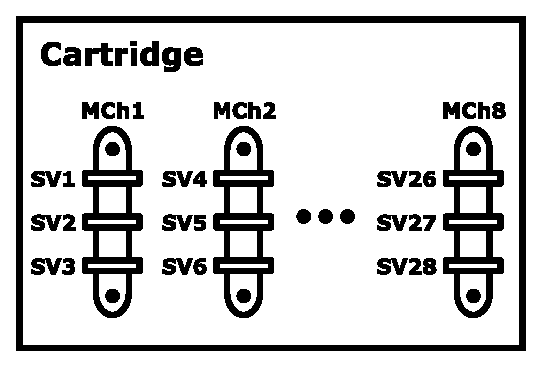
\includegraphics[width=.7\textwidth]{images/chapter_3/working_principle/cartridge.eps}
            \caption{Microfluidic channels and SV sensors diagram.}
            \label{figure:microchannels}
        \end{subfigure}\\
        \noalign{\bigskip}%
        \begin{subfigure}[c]{.48\textwidth}
            \centering
            \includegraphics[width=.7\textwidth]{working_principle/sensorpcb.png}
            \caption{Sensor chip bounded to the microfluidic channels and wire-bounded to the PCB (assay disposable cartridge).}
            \label{figure:microfluidic-pcb}
        \end{subfigure}
    \end{tabular}

    \caption{MFC system's cartridge.}
    \label{figure:microfluidic-channels}
\end{figure}

The detection mechanism in the \ac{MFC} platform has fundamental guidelines based on the constraints and particularities of in-flow magnetic detection \cite{Soares2019}. Figure \ref{figure:mfc-system-schematic} shows the diagram of an interaction between the \ac{MNP} flowing within a microfluidic channel and the magnetic field sensors. The permanent magnet magnetize the \ac{MNP}s attached to the analytes and pulls the beads closer to the sensor surface, acting as a vertical magnetophoresis. When in proximity to the sensor, the magnetic field produced by the particles is gradually picked up by the \ac{MR} sensors \cite{DiogoC_thesis}. 

\begin{figure}[!ht]
    \centering
    \includegraphics[width=.7\textwidth]{working_principle/mfc_system_schematic.png}
    \caption{Schematic representation of the MFC concept for magnetic particle detection (from Soares \textit{et al.} \cite{Soares2019}).}
    \label{figure:mfc-system-schematic}
\end{figure}

As explained in Section \ref{section:soa-mr-sensors}, the \ac{MR} sensor's resistance value increases or decreases, depending on the orientation and intensity of the magnetic field. Equation \ref{equation:mr-resistance-change} describes the resistance change behaviour of the \ac{MR} sensors. 
\begin{equation}
\label{equation:mr-resistance-change}
    R(H) = R_{NOM} + \Delta R(H) \quad [\Omega]
\end{equation}

\noindent
Whence $R_{NOM}$ is the sensor's resistance at $0T$ and $\Delta R(H)$ is the field-dependent resistance variation. Considering the target/\ac{MNP} conjugate behaves like a magnetic dipole, where the vector of field intensity has a different direction "in front" and "behind" the target in the sensor axis \cite{DiogoC_thesis}, ensuing the signal illustrated in Figure \ref{figure:mfc-system-schematic}. The interaction between sensors and particles results in a monocycle pulse if the excitation field is perpendicular to the particle. The signal negative flank occurrence before the positive is due to the \ac{MR} sensors direction axis.

% ############################################################################# Working Principle

% ############################################################################# System Overview
\section{System Overview}
\label{section:mfc-system}

As presented in Section \ref{section:soa-interfaces}, the systems that interfaces the sensors usually provide a fully analog path, from biasing to digital conversion. The interface system used in this dissertation brings continuity to a project developed by the \ac{INESC} research team to support a \ac{FC} application for early cancer detection. Whom, besides having a fully analog path, also has a fully digital path, from the raw data bitstream to the data measurement visualization.

Figure \ref{figure:mfc-block-diagram} illustrates the block diagram of the \ac{MFC} system. The interface consists of five main sections: biasing, amplification, filtering, digital conversion and digital signal processing. The biasing structure provides the demanded current for the \ac{MR} sensors to generate a signal when faced with a magnetic field. The amplification circuit boosts the low magnitude signal response of the sensors. The filtering increases the signal quality by removing unwanted components or features and using anti-aliasing filters. The \ac{ADC}, as the name implies, converts the analog signal into a digital representation. At last, the digital processing section enriches the system output signal, easing the event detection process that extracts the necessary information and displays it.

\begin{figure}[!ht]
    \centering
    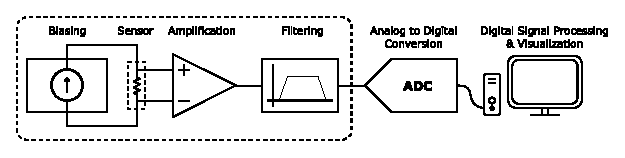
\includegraphics[width=.9\textwidth]{block_diagram.eps}
    \caption{Block diagram of the MFC system.}
    \label{figure:mfc-block-diagram}
\end{figure}

Several master thesis dissertations are being developed concurrently with this work, whose purpose is to improve the different sections that compose this system. The following paragraphs provide a brief explanation of the expected work by each of them.

\noindent
\textbullet \, Eng. João Faustino is responsible for the \ac{ADC} and all the electrical circuits that support it. The intention is to research a substitute system (\textit{e.g.} \ac{FPGA}) to the data acquisition board that limits the number of sensors and the sampling rate. In addition to his work, João will implement an oversampling technique while converting the output signal to digital, which ideally will lead to an improvement in the overall \ac{SNR} and resolution of the system. This section performs the first steps towards event detection, storing the events into a bitstream for preprocessing.

\noindent
\textbullet \, Eng. Diogo Bernardo work is between the \ac{ADC}, the digital signal processing and the visualization section. Diogo is researching and implementing advanced methods to improve the \ac{SNR} using \ac{DSP} methodologies. The idea is to have an independent system performing a real-time analysis of the \ac{MFC} bitstream output. The computer analysis consists of a machine learning algorithm that improves the success of the application event detection process.

\noindent
\textbullet \, Eng. Rita Ramos' dissertation thesis focused on the digital signal evaluation and visualization domain, specifically aiming to enhance the accurate detection of magnetically labeled analytes. Her work focused on improving a machine learning algorithm that utilizes neural networks \cite{10042449}. The purpose of this algorithm was to classify events based on whether they corresponded to magnetically tagged cells or clusters of magnetic particles employed in the tagging process.

The scope of this dissertation, highlighted by a dashed box in Figure \ref{figure:mfc-block-diagram}, encompasses all the circuitry involved in the analog path, including biasing architecture, signal amplification, and filtering. Additionally, it marks the initial stages of the digital path. The developed \ac{PCB} not only serves as an interface for the sensors but also to the acquisition board \ac{ADC}s and the \ac{FPGA}. The primary objective of this work is to significantly reduce the system-generated noise, making the \ac{MR} sensors the primary source of noise. Moreover, the new ultra-low noise cytometer platform will address several limitations present in the previous platform version.

\begin{figure}[!ht]
    \centering
    \includegraphics[width=.9\textwidth]{images/chapter_3/system.png}
    \caption{MFC system.}
    \label{figure:system}
\end{figure}

Figure \ref{figure:system} depicts the various boards comprising the system. The left \ac{PCB}, distinguished by its black solder mask, represents the cytometer platform developed as part of this work, which will be elaborated upon in the subsequent chapter. On the right, the blue \ac{PCB} represents the \ac{FPGA} (DE-10 Standard) and the acquisition board (THDB-ADA) selected by Eng. João Faustino for his project. At the top, the compact computer (Jetson-Nano) serves as the platform where Eng. Diogo Bernardo will execute his real-time machine learning algorithm.

% ############################################################################# System Overview

% ############################################################################# Interface Specifications
\section{Interface Specifications}
\label{section:mfc-specifications}

The specifications play a critical role in the design and development of electronic systems. By accurately defining and knowing the specifications, designers ensure the foundation for successful system integration. This section, will delve into the different specifications for the developed interface and explore their impact on the system performance and functionality.

As mentioned earlier, the cytometer platform attaches another \ac{PCB} (assay disposable cartridge) that accommodates the \ac{SV} sensor chip through wire bonding. This chip, developed at \ac{INESC}, incorporates 28 different \ac{MR} sensors arranged within 8 microfluidic channels. The nominal resistance (Equation \ref{equation:mr-resistance-change}) of these sensors may vary across different batches, with a range of approximately $\mathrm{500~\Omega}$ to $\mathrm{1.5~k\Omega}$. The biasing circuit, responsible for supplying a current to the passive sensors, must be capable of delivering at least $\mathrm{5~mA}$ when the sensors have the minimum nominal resistance. However, the circuit must also account for a potential increase in nominal resistance by at least $\mathrm{1~k\Omega}$, and ensure a stable current supply. When subjected to a magnetic field, the sensors generate a signal whose frequency primarily depends on the speed of the sample passing through the microfluidic channel. In a study \cite{DiogoC_thesis} conducted by Dr. Diogo Caetano, it was determined that for accurate flow rate measurements up to $\mathrm{30~\mu l/min}$, a minimum bandwidth of $\mathrm{100~kHz}$ is required. Additionally, the sensor response signal typically falls within the range of hundreds of microvolts. To amplify it to volt-level units and ensure maximum dynamic range for the \ac{ADC}s, the amplification circuit must have a gain of $\mathrm{10000~V/V}$.

An analog channel in the cytometer platform consists of a biasing circuit, an amplification circuit, and a filtering circuit. A minimum of 3 analog channels are required in the platform. This provides opportunities for experimentation and analysis. For example, utilizing two sensors within a microfluidic channel allows for redundant measurements. If both sensors experience a simultaneous resistance change caused by a magnetic particle, it confirms the presence of a particle rather than external interference. Moreover, including a third sensor in a channel without sample flow, serving as a reference channel, facilitates optimal particle detection by effectively eliminating common noise shared by all three sensors. Therefore, to fulfill this purpose, a minimum of 3 channels and 3 addressable sensors is required.

In addition to the analog path, the digital path of the signal also requires consideration. The DE-10 Standard \ac{FPGA}, used to control the cytometer and digital signal pre-processing, lacks built-in \ac{ADC}s. To overcome this limitation, an acquisition module called THDB-ADA is employed. However, this external card poses a significant constraint with only two available \ac{ADC}s. The \ac{ADC}s have a sampling rate of $\mathrm{65~MSPS}$ and cannot tolerate signals exceeding $\mathrm{2~Vp\textnormal{-}p}$.

\begin{table}[ht]
    \centering
    \caption{Front-end interface specifications.}
    \begin{small}
    \begin{tabular}{cc}
\toprule
Feature            & Specification                                              \\
\midrule                                             
$\mathrm{R_{sensor}}$   & $\mathrm{0.5 \geq R_{sensor} \leq 1.5~k\Omega}$       \\
$\mathrm{I_{bias}}$     & $\mathrm{I_{bias}(500\Omega) \geq 5~mA}$              \\
Bandwidth               & $\mathrm{100~kHz}$                                    \\
Signal Gain             & $\mathrm{10000~V/V}$                                  \\
Nº Channels             & $\mathrm{\geq 3}$                                     \\
Nº Sensors              & $\mathrm{3 \geq \textnormal{Sensors} \leq 28}$        \\
FPGA                    & DE-10 Standard                                        \\
Sampling Rate           & $\mathrm{\leq 65~MSPS}$                               \\
Nº ADCs                 & $\mathrm{2}$                                          \\
Output Voltage          & $\mathrm{\leq 2~Vp\textnormal{-}p}$                   \\
\bottomrule
\end{tabular}
    \end{small}
    \label{tab:specifications}
\end{table}

Table \ref{tab:specifications} presents an overview of the specifications discussed. The subsequent chapter will delve deeper into these specifications, exploring their significance and discussing how they were taken into account during the design process.

% ############################################################################# Interface Specifications

\clearpage
\thispagestyle{empty}
\cleardoublepage
